\subsection{Algoritmos exactos}
La \cref{tab:exactos} resume cuántas instancias resuelve cada algoritmo exacto con optimalidad probada. \hyvc{} resuelve 42 de las 46 instancias, frente a 20 de \textsf{DC-WH} y 17 de \textsf{DP-TD}. Las cuatro que no resuelve (bandas con $b=16$ y Barabási--Albert con $m=5$) tampoco las cerró CP-SAT en 30\,s con dos hilos, así que su óptimo sigue sin certificar.

\begin{table}[!htbp]\centering\small
\begin{tabular}{@{}lrrrrrr@{}}\toprule
 & \multicolumn{2}{c}{\textsf{DP-TD}} & \multicolumn{2}{c}{\textsf{DC-WH}} & \multicolumn{2}{c}{\hyvc} \\\cmidrule(lr){2-3}\cmidrule(lr){4-5}\cmidrule(l){6-7}
Familia & resueltas & $\bar t$ (s) & resueltas & $\bar t$ (s) & resueltas & $\bar t$ (s) \\\midrule
Erdős–Rényi $n{=}200$ & 6/15 & 0.00 & 6/15 & 4.32 & 15/15 & 0.42 \\
Erdős–Rényi $n{=}500$ & 0/4 & --- & 0/4 & --- & 4/4 & 0.37 \\
$k$-árbol parcial $n{=}300$ & 9/9 & 0.03 & 9/9 & 0.02 & 9/9 & 0.00 \\
Banda $n{=}400$ & 2/6 & 0.02 & 0/6 & --- & 4/6 & 0.46 \\
Barabási–Albert $n{=}1000$ & 0/6 & --- & 0/6 & --- & 4/6 & 0.00 \\
Trampa de Johnson & 0/3 & --- & 2/3 & 1.19 & 3/3 & 0.00 \\
Erdős–Rényi denso $n{=}60$ & 0/3 & --- & 3/3 & 0.13 & 3/3 & 0.14 \\
\midrule Total & 17/46 &  & 20/46 &  & 42/46 &  \\
\bottomrule\end{tabular}
\caption{Algoritmos exactos: instancias resueltas con optimalidad probada (límite 20\,s; \textsf{DP-TD} se rinde si el ancho supera 16) y tiempo medio sobre las resueltas.}\label{tab:exactos}\end{table}


Cada algoritmo base gana en su régimen y falla fuera de él, como predice la \cref{tab:secciones}. El divide y vencerás de Weigt y Hartmann resuelve en milisegundos los grafos que se fragmentan ($c=1$), tarda segundos en $c=2$ y no termina a partir de $c=3$, justo después de la transición en $c=e$ que describen los autores~\citep{weigt2001minimal} (\cref{fig:er}, derecha). La programación dinámica resuelve los $k$-árboles parciales y las bandas de ancho pequeño, pero la heurística de grado mínimo da anchos de 23 o más en todos los Erdős--Rényi con $c\ge 3$ y en todos los Barabási--Albert, y ahí ni siquiera arranca. \hyvc{} hereda ambos regímenes y además resuelve en menos de un segundo, en promedio, los Erdős--Rényi de $500$ vértices y los Barabási--Albert con $m\le 3$, que ningún algoritmo base cierra.

En los Erdős--Rényi densos ($n=60$, $c=15$) el divide y vencerás sin cotas y \hyvc{} empatan (0.13 frente a 0.14\,s). Ahí las reducciones no eliminan ningún vértice (\cref{tab:hyvc}) y la ventaja de \hyvc{} se limita a la poda por cotas.

\begin{figure}[!htbp]
\centering
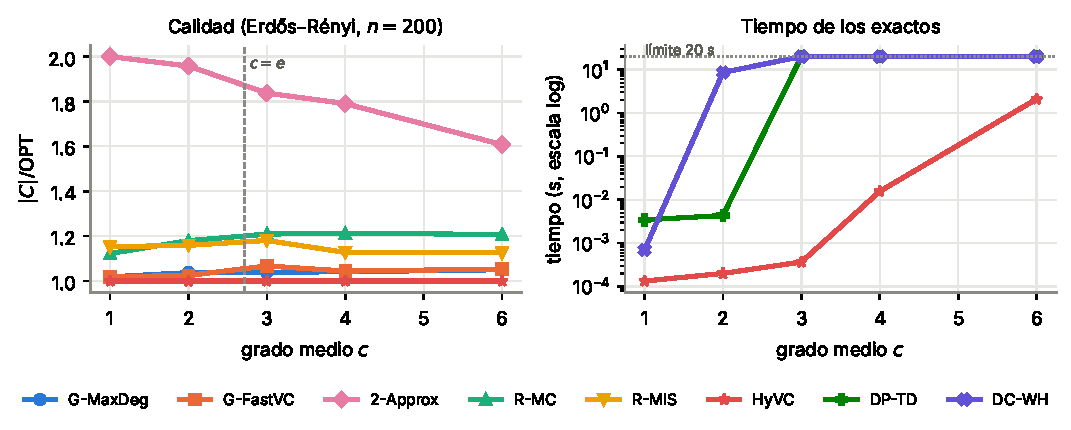
\includegraphics[width=\textwidth]{figs/er_quality_time.pdf}
\caption{Erdős--Rényi con $n=200$. Izquierda: razón media $|C|/\OPT$ de las heurísticas y de \hyvc. Derecha: tiempo medio de los algoritmos exactos; una corrida que no termina cuenta como 20\,s.}
\label{fig:er}
\end{figure}

\subsection{Calidad de las heurísticas}
La \cref{tab:calidad} compara la calidad de las heurísticas con el óptimo. La construcción de FastVC es la mejor heurística en promedio (razón 1.037) y la única que no cae en la trampa de Johnson, donde el greedy de grado máximo llega a $2.95$ veces el óptimo ($k=80$: 288 frente a 80). Fuera de esa familia, el greedy de grado máximo y FastVC quedan entre un 0.5\,\% y un 5\,\% por encima del óptimo. Fuera de la trampa, los dos aleatorizados con garantía de razón $2$ en esperanza (\textsf{R-MC} con $\gamma=1$ y \textsf{R-MIS}) quedan entre un 4\,\% y un 26\,\% por encima, y el matching maximal casi duplica el óptimo, como era de esperar.

\begin{table}[!htbp]\centering\scriptsize\setlength{\tabcolsep}{3.5pt}
\begin{tabular}{@{}lrrrrrr@{}}\toprule
Familia & \textsf{G-MaxDeg} & \textsf{G-FastVC} & \textsf{2-Approx} & \textsf{R-MC} & \textsf{R-MIS} & \textsf{HyVC} \\\midrule
Erdős–Rényi $n{=}200$ & 1.037 & 1.042 & 1.839 & 1.186 & 1.149 & 1.000 \\
Erdős–Rényi $n{=}500$ & 1.050 & 1.046 & 1.864 & 1.242 & 1.144 & 1.000 \\
$k$-árbol parcial $n{=}300$ & 1.005 & 1.023 & 1.891 & 1.221 & 1.149 & 1.000 \\
Banda $n{=}400$ & 1.036$^{4/6}$ & 1.046$^{4/6}$ & 1.416$^{4/6}$ & 1.170$^{4/6}$ & 1.092$^{4/6}$ & 1.000$^{4/6}$ \\
Barabási–Albert $n{=}1000$ & 1.025$^{4/6}$ & 1.046$^{4/6}$ & 1.908$^{4/6}$ & 1.256$^{4/6}$ & 1.185$^{4/6}$ & 1.000$^{4/6}$ \\
Trampa de Johnson & 2.950 & 1.000 & 2.000 & 1.717 & 2.258 & 1.000 \\
Erdős–Rényi denso $n{=}60$ & 1.043 & 1.050 & 1.281 & 1.108 & 1.043 & 1.000 \\
\midrule Todas & 1.168 & 1.037 & 1.790 & 1.237 & 1.218 & 1.000 \\
\bottomrule\end{tabular}
\caption{Razón media $|C|/\OPT$ (1.000 = óptimo). El superíndice $a/b$ indica que el algoritmo solo tiene óptimo certificado en $a$ de las $b$ instancias; la media se calcula sobre esas $a$. Los exactos \textsf{DP-TD} y \textsf{DC-WH} se omiten: cuando terminan su razón es 1 (ver \cref{tab:exactos}).}\label{tab:calidad}\end{table}


En las cuatro instancias que nadie resolvió, la cubierta \emph{anytime} de \hyvc{} queda entre un 3.0\,\% y un 3.9\,\% por encima de la mejor solución de CP-SAT. Nunca es peor que la mejor heurística voraz y es estrictamente mejor en tres de las cuatro (311 frente a 314, 606 frente a 611 y 615 frente a 618). Es un resultado modesto: cuando la búsqueda exacta no termina, \hyvc{} no hace búsqueda local y se queda prácticamente con su cota superior inicial.

\subsection{El parámetro $\gamma$ del greedy aleatorizado}
La \cref{fig:gamma} reproduce el comportamiento que reportan Gao et al.~\citep{gao2018randomized}. Con $\gamma=1$, una sola corrida sobre la trampa de Johnson da $1.99$ veces el óptimo, en línea con la garantía de razón $2$ en esperanza. Al subir $\gamma$ la calidad mejora rápidamente, y con $\gamma\ge 8$ y $16$ corridas se alcanza el óptimo de la trampa (80), donde el greedy determinista obtiene 288. En los grafos aleatorios, repetir 16 veces mejora la razón como mucho en $9$ puntos porcentuales; subir $\gamma$ pesa mucho más que repetir.

\begin{figure}[!htbp]
\centering
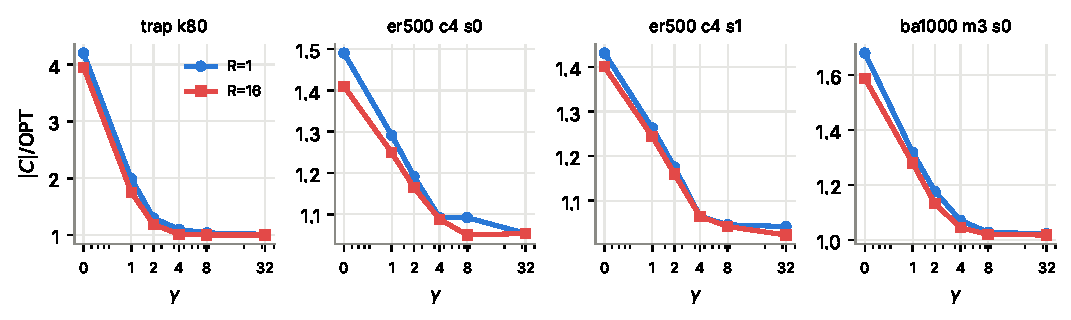
\includegraphics[width=\textwidth]{figs/gamma.pdf}
\caption{Greedy aleatorizado $\deg^\gamma$: razón $|C|/\OPT$ en función de $\gamma$, con una corrida ($R=1$) y con la mejor de 16 ($R=16$).}
\label{fig:gamma}
\end{figure}

\subsection{Qué sección hace el trabajo: ablación}
La \cref{tab:hyvc} muestra dónde trabaja \hyvc{} en cada familia, y la \cref{tab:ablacion} y la \cref{fig:ablacion} apagan una sección a la vez, con un límite de 10\,s.

\begin{table}[!htbp]\centering\small
\begin{tabular}{@{}lrrrr@{}}\toprule
Familia & núcleo tras reducir & comp.\ a PD & comp.\ a B\&R & nodos B\&R (media) \\\midrule
Erdős–Rényi $n{=}200$ & 23.0\% & 0 & 5 & 538 \\
Erdős–Rényi $n{=}500$ & 23.3\% & 0 & 2 & 391 \\
$k$-árbol parcial $n{=}300$ & 0.0\% & 0 & 0 & 0 \\
Banda $n{=}400$ & 93.7\% & 4 & 3 & 59 \\
Barabási–Albert $n{=}1000$ & 33.3\% & 0 & 2 & 4771 \\
Trampa de Johnson & 0.0\% & 0 & 0 & 0 \\
Erdős–Rényi denso $n{=}60$ & 100.0\% & 0 & 3 & 150 \\
\bottomrule\end{tabular}
\caption{Qué sección de \hyvc{} hace el trabajo: fracción de vértices que sobrevive a las reducciones, componentes despachadas a programación dinámica o a branch \& reduce, y nodos de búsqueda.}\label{tab:hyvc}\end{table}


\begin{itemize}
  \item \textbf{Reducciones} (Ásgeirsson--Stein, Akiba--Iwata). Es la sección más importante. Resuelve por completo los $k$-árboles parciales y la trampa de Johnson, deja núcleos del 23\,\% en los Erdős--Rényi y del 33\,\% en los Barabási--Albert, y sin ella \hyvc{} pasa de 10/10 a 6/10 instancias exactas en Erdős--Rényi y de 4/6 a 0/6 en Barabási--Albert.
  \item \textbf{Programación dinámica} (Bannach--Berndt, Alber et al.). Es decisiva en las bandas: sin ella, \hyvc{} pasa de 4/6 a 1/6 instancias exactas y de 37 a más de 27\,000 nodos de búsqueda en promedio. En los Erdős--Rényi tiene un costo neto: estimar $\kappa(H)$ en cada nodo hace que \hyvc{} completo tarde 0.37\,s frente a 0.21\,s sin PD.
  \item \textbf{División en componentes} (Weigt--Hartmann) y \textbf{cota Monte Carlo} (Gao et al.). En estas instancias no tienen un efecto medible: apagarlas no cambia ni el número de instancias exactas ni el tiempo más allá del ruido. Después de las reducciones, los núcleos son casi siempre una sola componente grande que la búsqueda no alcanza a fragmentar en 10\,s, y la cota superior voraz ya está a pocos vértices del óptimo, así que la búsqueda pasa casi todo su tiempo probando la cota inferior y no mejorando la superior.
\end{itemize}

\begin{table}[!htbp]\centering\small
\begin{tabular}{@{}llrrr@{}}\toprule
Familia & Variante & $\bar t$ (s) & exactas & nodos \\\midrule
Erdős–Rényi $n{=}200$ & HyVC completo & 0.37 & 10/10 & 481 \\
 & sin reducciones & 5.38 & 6/10 & 44 \\
 & sin DP & 0.21 & 10/10 & 561 \\
 & sin division & 0.40 & 10/10 & 484 \\
 & sin Monte Carlo & 0.37 & 10/10 & 486 \\
\addlinespace
Banda $n{=}400$ & HyVC completo & 3.72 & 4/6 & 37 \\
 & sin reducciones & 3.82 & 4/6 & 40 \\
 & sin DP & 8.50 & 1/6 & 27573 \\
 & sin division & 3.73 & 4/6 & 34 \\
 & sin Monte Carlo & 3.74 & 4/6 & 39 \\
\addlinespace
Barabási–Albert $n{=}1000$ & HyVC completo & 3.36 & 4/6 & 2572 \\
 & sin reducciones & 10.26 & 0/6 & 238 \\
 & sin DP & 3.36 & 4/6 & 3840 \\
 & sin division & 3.36 & 4/6 & 2351 \\
 & sin Monte Carlo & 3.35 & 4/6 & 2307 \\
\bottomrule\end{tabular}
\caption{Ablación: se apaga una sección de \hyvc{} a la vez (límite 10\,s). Si una variante no termina, aporta 10\,s a la media.}\label{tab:ablacion}\end{table}


\begin{figure}[!htbp]
\centering
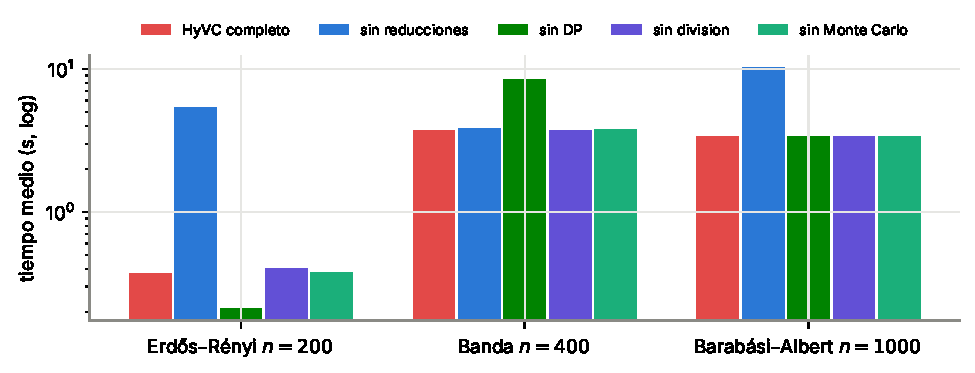
\includegraphics[width=0.85\textwidth]{figs/ablation.pdf}
\caption{Ablación: tiempo medio de \hyvc{} al apagar una sección (escala logarítmica, límite 10\,s).}
\label{fig:ablacion}
\end{figure}

\subsection{Amenazas a la validez}
Todas las implementaciones, \hyvc{} incluido, están en Python. Los tiempos absolutos no son comparables con implementaciones en C++ como las de los artículos originales; solo lo son las comparaciones relativas dentro de este trabajo. Las instancias son sintéticas y de tamaño moderado (hasta 1000 vértices). Usamos 2 o 3 semillas por configuración, así que las diferencias pequeñas de tiempo no son significativas. El ancho de árbol se estima con una sola heurística (grado mínimo); una mejor descomposición ampliaría el régimen de la PD. Por último, los parámetros de \hyvc{} ($\kappa_{\max}$, el tope interno, $\gamma$ y $R$) se fijaron a mano, y la elección de $\gamma=2$ es subóptima según la \cref{fig:gamma}.
